\documentclass[12pt]{article}
\usepackage{graphicx,float}
\usepackage{listings}
\usepackage{xcolor}
\graphicspath{{./fig/}}

\definecolor{codegreen}{rgb}{0,0.6,0}
\definecolor{codegray}{rgb}{0.5,0.5,0.5}
\definecolor{codepurple}{rgb}{0.58,0,0.82}
\definecolor{backcolour}{rgb}{0.95,0.95,0.92}


\lstdefinelanguage{SPICE}{
  keywords={tran,ac,dc,subckt,meas,plot,print,control,run,end,endc, hardcopy},
  morecomment=[l]{*},
  morecomment=[l]{\$},
  morecomment=[s]{/*}{*/},
  morestring=[b]',
  morestring=[b]",
  ndkeywords={r,r1,r2,r3,r4,r5,l,l1,l2,l3,l4,l5,c,c1,c2,c3,c4,c5,v,vin,m,m1,m2,m3,m4,m5,d,d1,d2,d3,d4,d5,vdb, pulse,sin,i,pwl,exp},
  keywordstyle=\color{blue}\bfseries,
  ndkeywordstyle=\color{codegreen}\bfseries,
  identifierstyle=\color{black},
  commentstyle=\color{purple}\ttfamily,
  stringstyle=\color{red}\ttfamily,
  sensitive=true
}

\lstdefinestyle{mystyle}{
	backgroundcolor=\color{backcolour},   
    commentstyle=\color{codegreen},
    keywordstyle=\color{magenta},
    numberstyle=\tiny\color{codegray},
    stringstyle=\color{codepurple},
    basicstyle=\ttfamily\footnotesize,
    breakatwhitespace=false,         
    breaklines=true,                 
    captionpos=b,                    
    keepspaces=true,                 
    numbers=left,                    
    numbersep=5pt,                  
    showspaces=false,                
    showstringspaces=false,
    showtabs=false,                  
    tabsize=4
}

\lstset{style=mystyle}


% Title[Enter title of the experiment here]
\title{EE230: Lab-4\\
Simple Application Circuits}

% Author[Enter details of author here]
\author{Prateek Garg, 20D070060}

% begin the document.
\begin{document}
\noindent
% make a title page.[this creates title page]
\maketitle

\section{Overview of the experiment} %[This segment creates Section as seen in document]

\subsection{Aim of the experiment}%[This segment creates sebsections under the same section]
The aim of the experiment is to understand and simulate a photo diode using an Op-Amp and a 3 Op-Amp based instrumentation amplifier.
\subsection{Methods}
We start by analysing the circuits and then simulating in ngspice to check against theoretical expectations.  
\section{Design}
\subsection*{Photo Diode}
\begin{figure}[H]
    \centering
    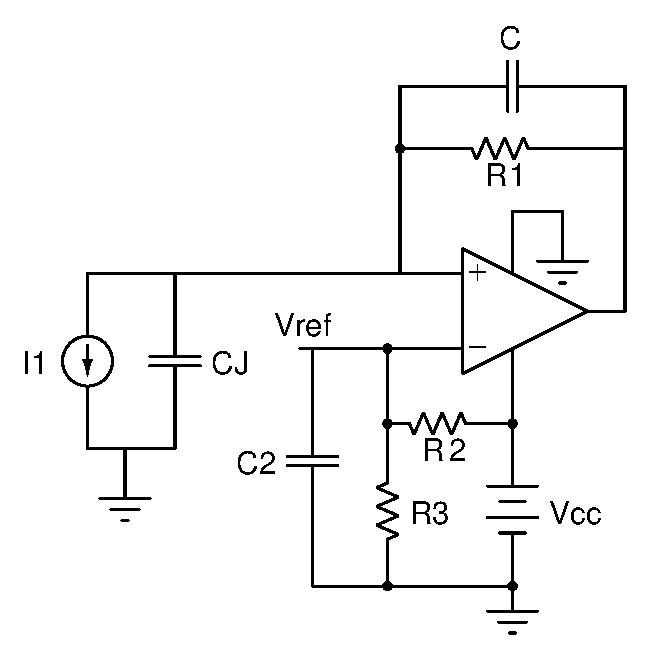
\includegraphics{photodiode.eps}
    \caption{Photodiode}
\end{figure}
The circuit diagram of a Photo Diode is shown above. It uses a current source and a capacitor to simulate a Photodiode model and then uses its outputs as inputs to the Op-Amp.\newline
The $V_{cc}$ of the Op-Amp is grounded and the $V_{ee}$ is equal to 5V.

\subsection*{Instrumentation Amplifier}

\begin{figure}[H]
    \centering
    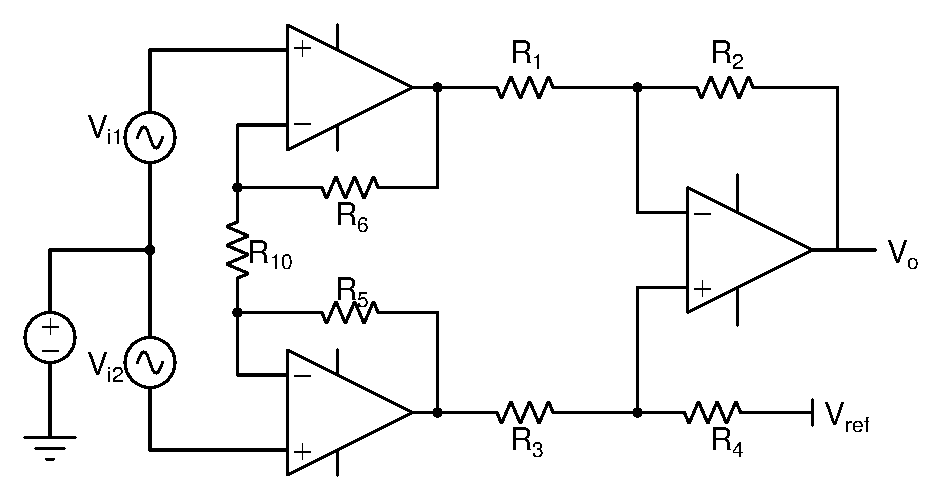
\includegraphics{instrumentation.eps}
    \caption{Instrumentation Amplifier}
\end{figure}
The circuit diagram of instrumentation amplifier is shown above. \newline 
An instrumentation amplifier is a type of differential amplifier that has been outfitted with input buffer amplifiers, which eliminate the need for input impedance matching and thus make the amplifier particularly suitable for use in measurement and test equipment. \newline
Additional characteristics include very low DC offset, low drift, low noise, very high open-loop gain, very high common-mode rejection ratio, and very high input impedance. Instrumentation amplifiers are used where great accuracy and stability of the circuit both short- and long-term are required.
\newline
The gain of the amplifier is given:

\begin{equation}
    A_{v}=\left(1+\frac{2R_{6}}{R_{10}}\right)\frac{R_3}{R_2}
\end{equation}

\section{Simulation results}

\subsection{Photo Diode}
\subsubsection{Code snippet}
\lstinputlisting[language=SPICE]{../Q1-a.cir}
\lstinputlisting[language=SPICE]{../Q1-b.cir}

\subsection{Instrumentation Amplifier}
\subsubsection{Code snippet}
\lstinputlisting[language=SPICE]{../Q2-b.cir}
\lstinputlisting[language=SPICE]{../Q2-c.cir}

\subsubsection{Simulation results}
\textbf{\large Photo Diode}
\begin{figure}[H]
  \begin{center}
    \makebox[0.8\textwidth]{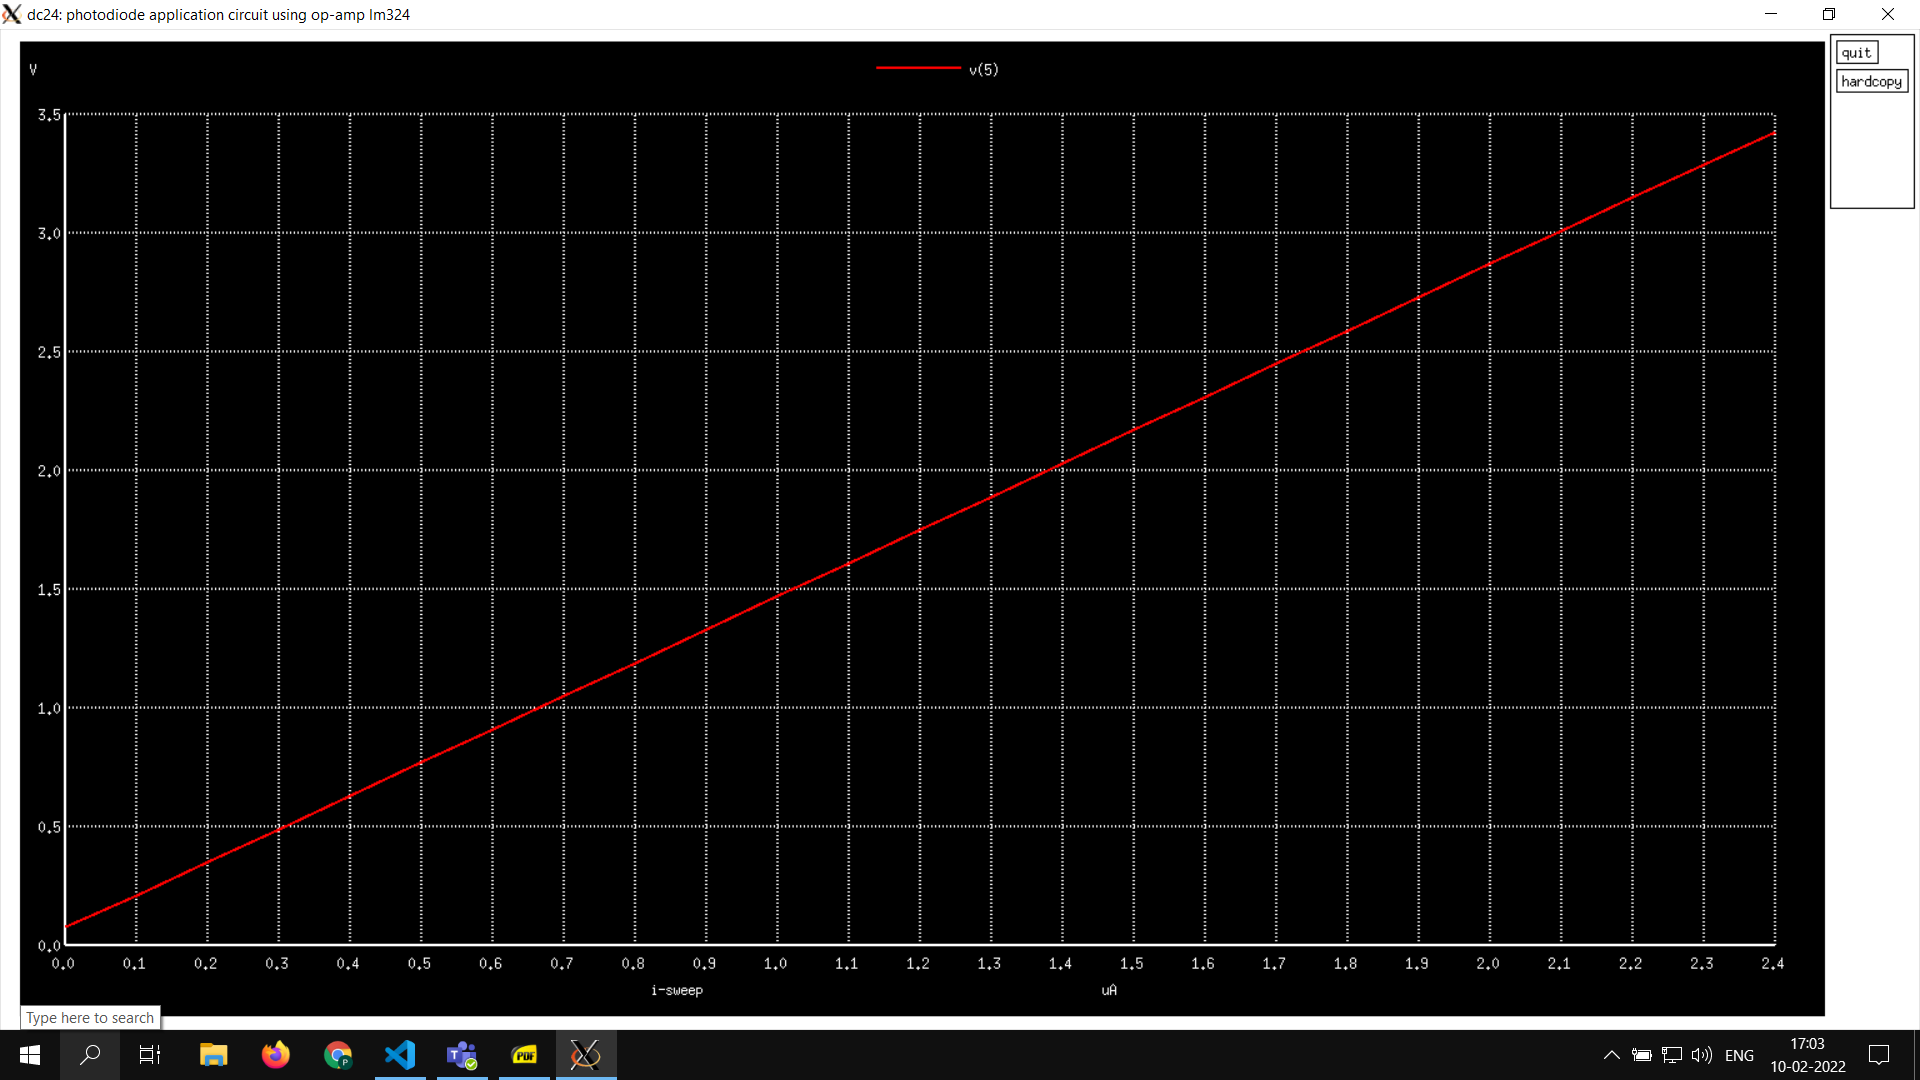
\includegraphics[width=0.8\paperwidth]{q1-a.png}}
\end{center}
\end{figure}

\begin{figure}[H]
    \begin{center}
      \makebox[0.8\textwidth]{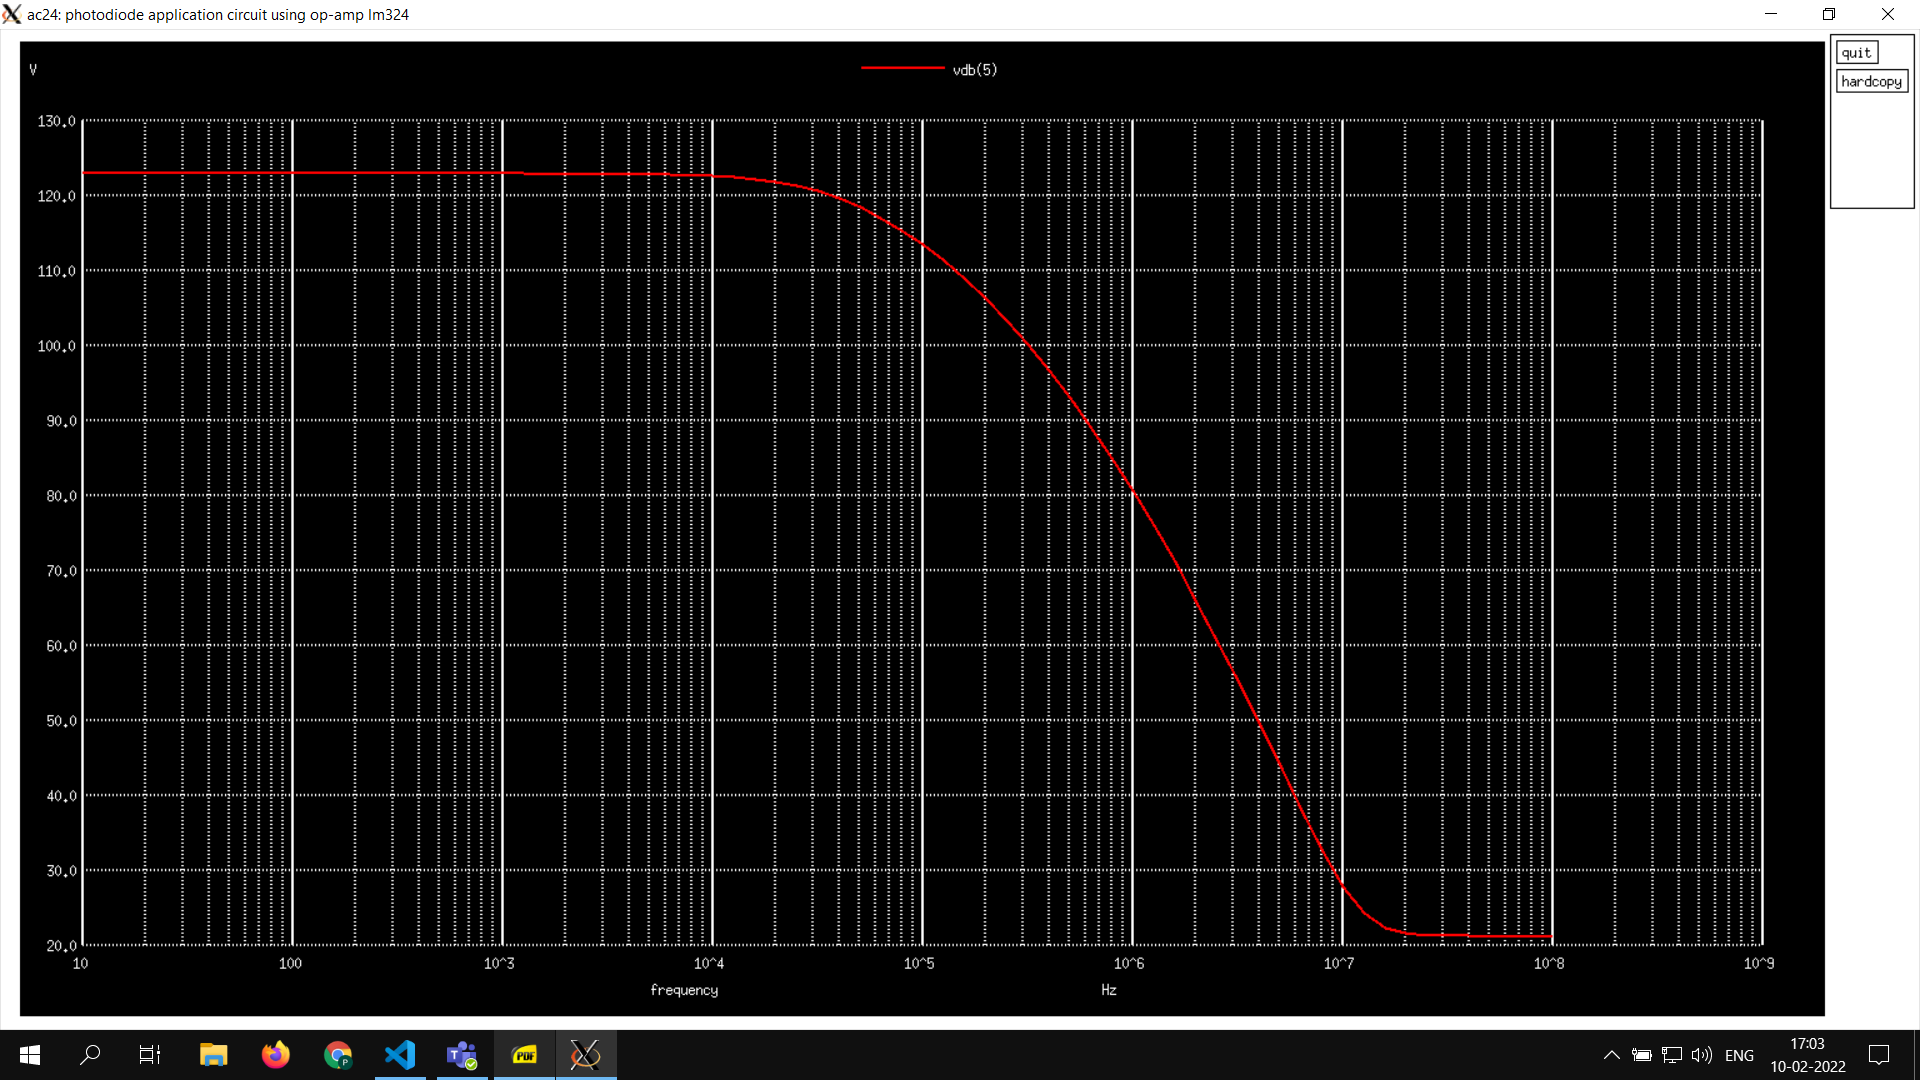
\includegraphics[width=0.8\paperwidth]{q1-b.png}}
\end{center}
\end{figure}

\textbf{\large Instrumentation Amplifier}
\begin{figure}[H]
  \begin{center}
    \makebox[0.8\textwidth]{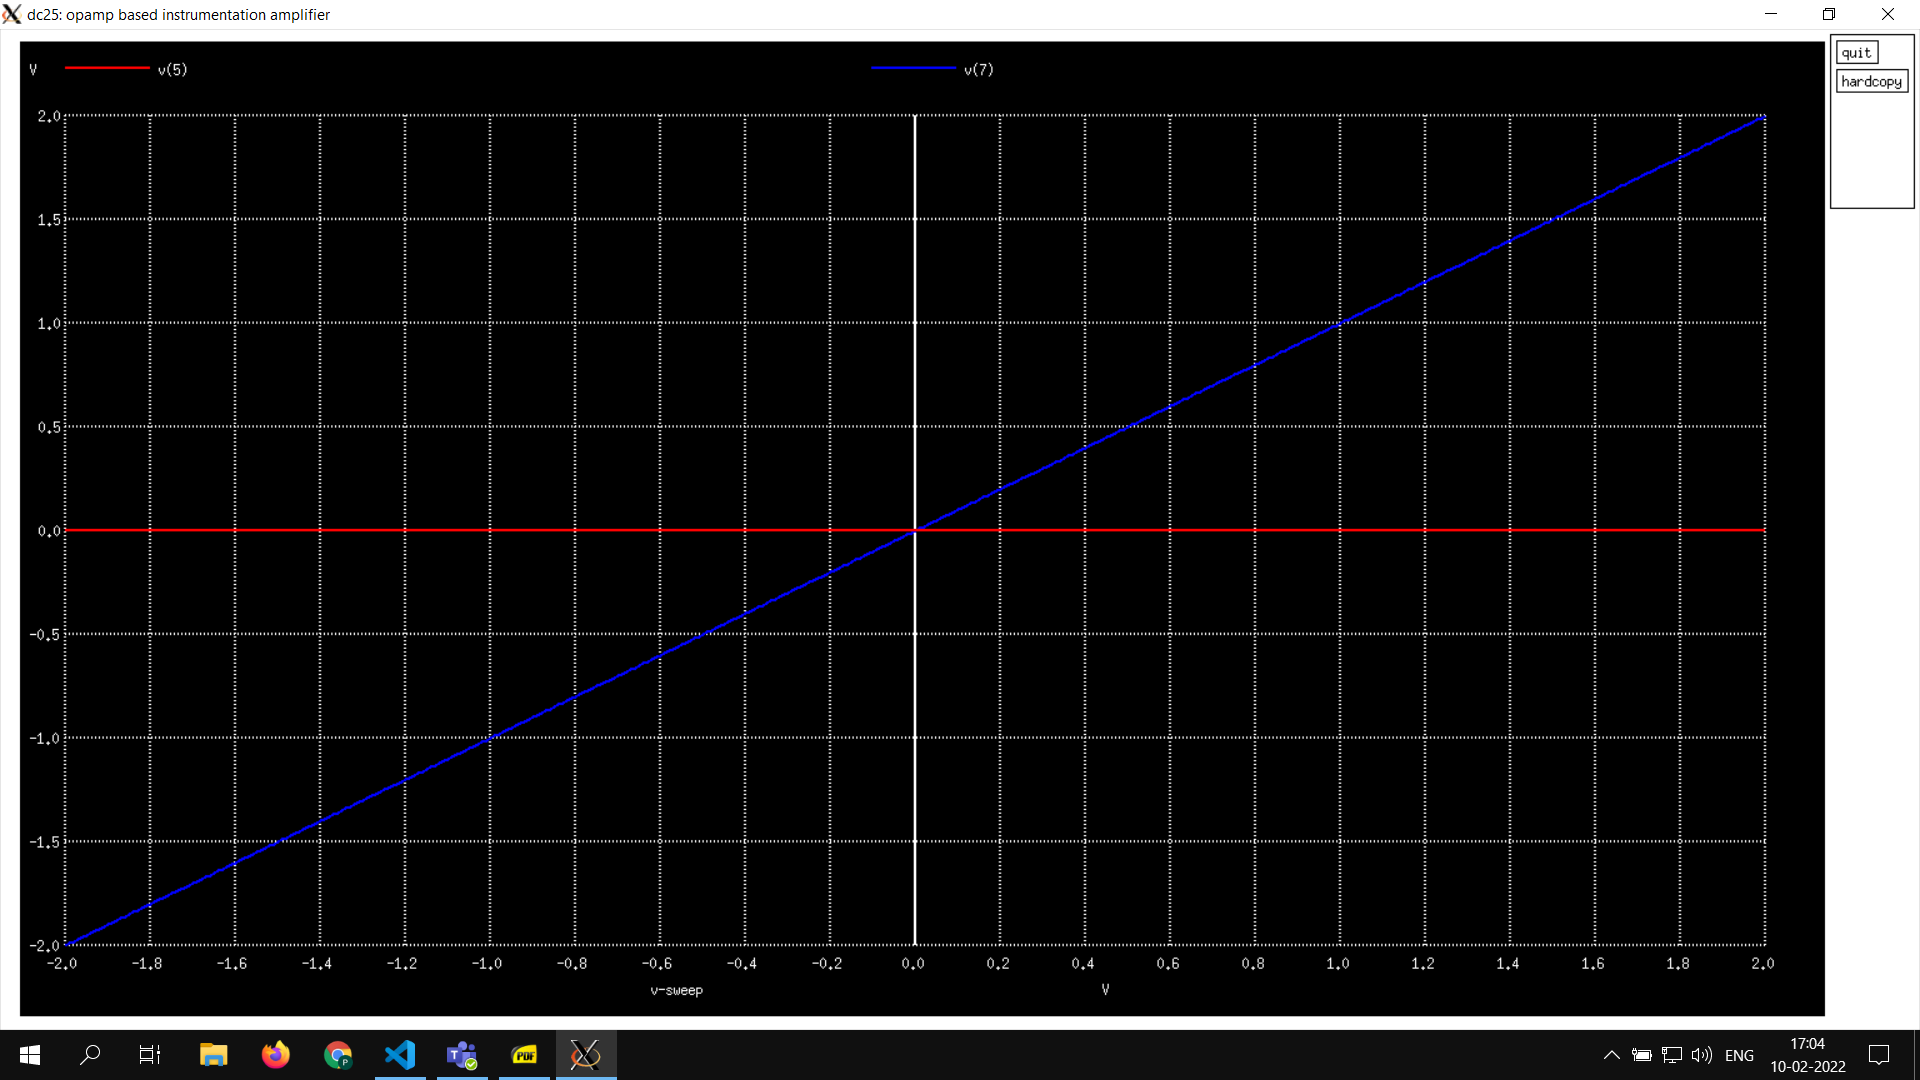
\includegraphics[width=0.8\paperwidth]{q2-b.png}}
\end{center}
\end{figure}

\begin{figure}[H]
    \begin{center}
      \makebox[0.8\textwidth]{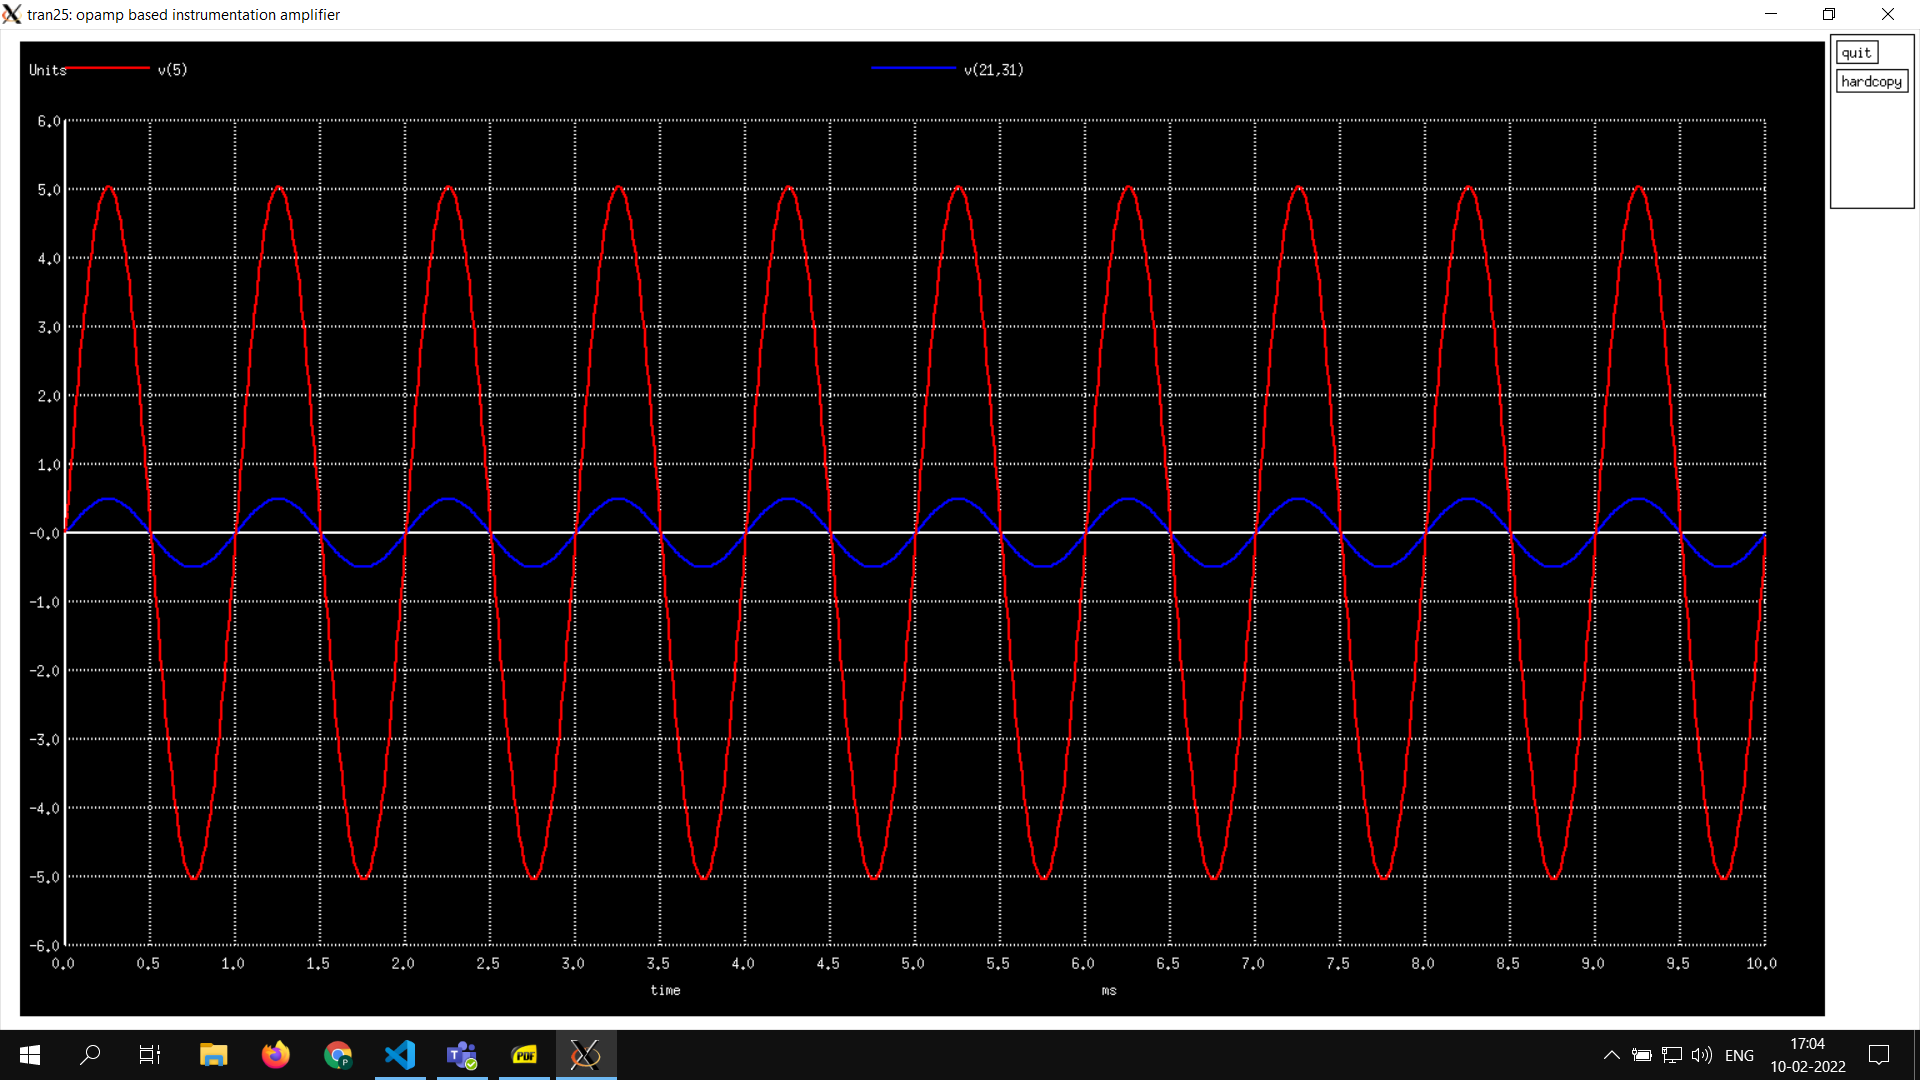
\includegraphics[width=0.8\paperwidth]{q2-c.png}}
  \end{center}
  \end{figure}

\section{Experiment completion status}
All the sections were completed
\end{document}
